\documentclass[a4paper, 12pt]{report}
\usepackage[utf8]{inputenc}
\usepackage[T1]{fontenc}
\usepackage[french]{babel}
\usepackage{graphicx}
\usepackage{amsmath}
\usepackage{hyperref}
\usepackage{geometry}
\usepackage{comment}
\usepackage{float}
\usepackage{listings}
\usepackage[none]{hyphenat}
\usepackage{fancyhdr}
\usepackage{datetime}
\usepackage{tocloft}
\usepackage{chngcntr}
\usepackage{titlesec}
\usepackage{caption}
\usepackage{etoolbox}
\usepackage{csquotes}
\usepackage[bottom]{footmisc}
\usepackage{tocloft}
\usepackage{titlesec}
\usepackage{chngcntr}
\usepackage{times}
\usepackage{enumitem}
\usepackage{pdfpages}
\usepackage[nameinlink]{cleveref}
%\usepackage{draftwatermark} % Pour ajouter un watermark
\usepackage{lipsum} % Pour générer du texte d'exemple
\usepackage[toc,numberedsection=autolabel,acronym,nonumberlist]{glossaries} %,nonumberlist % pour ne pas afficher les numéros de page dans le glossaire
\usepackage[backend=biber,style=apa]{biblatex}
\addbibresource{bibliographie.bib}
\geometry{left=2.5cm, right=2.5cm, top=2.5cm, bottom=2.5cm}
\makeglossaries % pour update de glossaire 4 commandes : pdflatex main.tex, makeglossaries main, pdflatex main.tex, pdflatex main.tex


\begin{document}
\sloppy


\titleformat{\chapter}[hang]
    {\normalfont\huge\bfseries}{\thechapter}{1em}{}

\newbool{couverture}
\booltrue{couverture}
\titlespacing*{\chapter}
    {0pt}
    {0pt}
    {20pt}
\setlength\cftbeforetoctitleskip{0pt}
\setlength\cftbeforelottitleskip{0pt}
\setlength\cftbeforeloftitleskip{0pt}

\setlength\cftaftertoctitleskip{20pt}
\setlength\cftafterlottitleskip{20pt}
\setlength\cftafterloftitleskip{20pt}

% Configuration du watermark si besoin décommenter les lignes suivantes
%\SetWatermarkText{Confidential}
%\SetWatermarkScale{1.5}
%\SetWatermarkColor{red}
%\SetWatermarkAngle{45}

\fancypagestyle{couverture}{
    \fancyhf{}
    \fancyhead[L]{\includegraphics[width=8cm]{img/logo_hehbe_tech.png}} 
    \fancyhead[R]{\vspace{1.8cm}\textbf{Année académique 20xx-20xx}} 
    \fancyfoot[L]{Promoteur : Nom Prénom} 
    \fancyfoot[R]{Étudiant : Nom Prénom} 
    \fancyfoot[C]{} 
    \renewcommand{\headrulewidth}{0pt} 
    \renewcommand{\footrulewidth}{0pt} 
}

\fancypagestyle{page_de_garde}{
    \fancyhf{}
    \fancyhead[L]{\includegraphics[width=8cm]{img/logo_hehbe_tech.png}} 
    \fancyhead[R]{\vspace{1.8cm}\textbf{Année académique 20xx-20xx}} 
    \fancyfoot[L]{Promoteur : Nom Prénom} 
    \fancyfoot[C]{\monthname~\the\year}
    \fancyfoot[R]{Étudiant : Nom Prénom}
    \renewcommand{\headrulewidth}{0pt} 
    \renewcommand{\footrulewidth}{0pt}
}

\fancypagestyle{plain}{
    \fancyhf{}
    \fancyhead[L]{\includegraphics[width=0.15\textwidth]{img/logo_hehbe_tech.png}}
    \fancyhead[R]{\vspace{0.1cm}\textbf{Année académique 2024-2025}}
    \fancyfoot[R]{Page \thepage}
    \renewcommand{\headrulewidth}{0.1pt}
    \renewcommand{\footrulewidth}{0pt}
}

\pagestyle{fancy}
\fancyhf{}
\renewcommand{\footrulewidth}{0pt}
\renewcommand{\headrulewidth}{0.1pt}
\fancyhead[L]{\includegraphics[width=0.15\textwidth]{img/logo_hehbe_tech.png}}
\fancyhead[R]{\vspace{0.1cm}\textbf{Année académique 2024-2025}}
\fancyfoot[R]{Page \thepage}
\headsep = 1.5cm
\textheight = 24cm

\newcommand{\garde}{
    \ifbool{couverture}{\thispagestyle{couverture}}{\thispagestyle{page_de_garde}}
    \vspace*{2cm}
    \begin{center}    
        {\large \textbf{HAUTE ECOLE DE LA COMMUNAUTE FRANCAISE EN HAINAUT}}\\
        {\large Département des Sciences et Technologies}\\
        {\large 8A Avenue Victor Maistriau -- 7000 Mons}
    \end{center}
    \vspace{3cm}
    \begin{center}
        \fboxrule=0.3mm
        \fbox{
            \parbox{\textwidth}{
                \vspace{1cm}
                \centering
                \textbf{Lorem ipsum dolor sit amet, consectetur adipiscing elit. Vivamus lacinia odio vitae}
                \vspace{1cm}
            }
        }
    \end{center}
    \vspace{1.5cm}
    \begin{center}
        \normalsize{\textit{Projet de fin d'études réalisé en vue de l'obtention du titre de Bachelier en Informatique Orientation réseaux \& télécommunications option développement ou sécurité}}
    \end{center}
    \vspace{5cm}
    \date{}
}

\crefname{section}{section}{sections}
\crefname{chapter}{chapitre}{chapitres}
\newcommand{\fullref}[1]{cf. chapitre~\ref{#1}, page~\pageref{#1}}

\garde
\newpage
\thispagestyle{empty} 
\mbox{}
\newpage
\pagenumbering{arabic}
\boolfalse{couverture}
\garde
\chapter*{}
 % Supprime le numéro de page pour cette section

\vfill % Pousse le contenu vers le bas

\hfill % Aligne le contenu à droite
\begin{minipage}{0.5\textwidth} % Définit une largeur pour le texte
    {\itshape % Utilisation de \itshape pour appliquer l'italique à tout le contenu
        Je tiens à exprimer ma profonde gratitude à toutes les personnes qui ont contribué, de près ou de loin, à la réalisation de ce projet.

        Je remercie tout particulièrement :
        

        \vspace{1cm}

}
\end{minipage}

\vspace{1cm} % Ajoute un espace en bas si nécessaire

\input{chapter/tables.tex}
\addcontentsline{toc}{chapter}{Abréviations}
\glsaddall
\printglossary[type=\acronymtype, title={Liste des abréviations}]


\chapter{Abstract Étendu}
\label{chap:abstract}

\lipsum[1-2]

\section{Lorem Ipsum}
\lipsum[3-4]

\section{Références}
\printbibliography[type=book,heading=none]
\printbibliography[type=online,heading=none]
\input{chapter/Introduction.tex}
\newpage
\chapter*{Commandes}


Voici les différents paramètres pour mettre en forme le texte : 

Exemple: \textbf{Texte en gras}.
\begin{verbatim}
\textbf{texte} : Pour mettre le texte en gras.
\end{verbatim}

Exemple: \textit{Texte en italique}.
\begin{verbatim}
\textit{texte} : Pour mettre le texte en italique.
\end{verbatim}

Exemple: \underline{Texte souligné}.
\begin{verbatim}
\underline{texte} : Pour souligner le texte.
\end{verbatim}

Exemple: \texttt{Texte en code}.
\begin{verbatim}
\texttt{texte} : Pour représenter du code.
\end{verbatim}

Exemple: \textsc{Texte en petites majuscules}.
\begin{verbatim}
\textsc{texte} : Pour mettre le texte en petites majuscules.
\end{verbatim}

Exemple: \textsf{Texte sans empattement}.
\begin{verbatim}
\textsf{texte} : Pour un style sans empattement.
\end{verbatim}

Exemple: \textsl{Texte en italique}.
\begin{verbatim}
\textsl{texte} : Pour mettre le texte en italique (autre variante).
\end{verbatim}

Exemple: \textbf{\textit{Texte en gras et italique}}.
\begin{verbatim}
\textbf{\textit{texte}} : Pour mettre le texte en gras et italique.
\end{verbatim}

Exemple: \textbf{\underline{Texte en gras et souligné}}.
\begin{verbatim}
\textbf{\underline{texte}} : Pour mettre le texte en gras et souligné.
\end{verbatim}

Exemple: \textit{\underline{Texte en italique et souligné}}.
\begin{verbatim}
\textit{\underline{texte}} : Mettre le texte en italique et souligné.
\end{verbatim}

Exemple: $x^6$ ou $H_2O$ RTBF$^{87}$.
\begin{verbatim}
Texte en exposant : Puissances/indices, ex: $x^6$ ou $H_2O$ RTBF$^{87}$.
\end{verbatim}

Exemple: \hyperlink{RTBF}{RTBF}$^{\hyperlink{RTBF}{87}}$.
\begin{verbatim}
Texte avec lien : \hyperlink{RTBF}{RTBF}$^{\hyperlink{RTBF}{87}}$.
\end{verbatim}

Exemple: Référence\textsuperscript{\cite{ref1}}.
\begin{verbatim}
Référence\textsuperscript{\cite{ref1}} : Ajouter des références.
\end{verbatim}

\begin{verbatim}
    \raggedright : Pour eviter de couper les mots en fin de ligne
\end{verbatim}






\newpage
\chapter{chap1}
\label{chap:chap1}
\lipsum[1-2]
\gls{gpu}



\begin{figure}[!ht]
    \centering
    \includegraphics[width=8cm]{img/logo_hehbe_tech.png}
    \caption{Logo de la HEHBE}
    \label{fig:logo heh tech}
\end{figure}
\chapter{Bibliographie}

\nocite{*}

\section{Livres}
\printbibliography[type=book,heading=none]

\section{Articles}
\printbibliography[type=article,heading=none]



\printglossary

\newglossaryentry{exemple}{
    name=Exemple,
    description={Un exemple est une illustration ou un cas particulier utilisé pour expliquer ou clarifier un concept},
    type=main
}

\newglossaryentry{latex}{
    name=LaTeX,
    description={Un système de composition de documents pour produire des documents de haute qualité},
    type=main
}

\newglossaryentry{api}{
    name=API,
    description={Application Programming Interface, une interface qui permet à des applications de communiquer entre elles},
    type=main
}


% Définition des abréviations
\newacronym{gpu}{GPU}{Unité de Traitement Graphique}
\newacronym{cpu}{CPU}{Unité Centrale de Traitement}
\newacronym{api}{API}{Interface de Programmation d'Application}

\newpage
\refstepcounter{chapter}
\addcontentsline{toc}{chapter}{\protect\numberline{\thechapter}Cahier des charges}
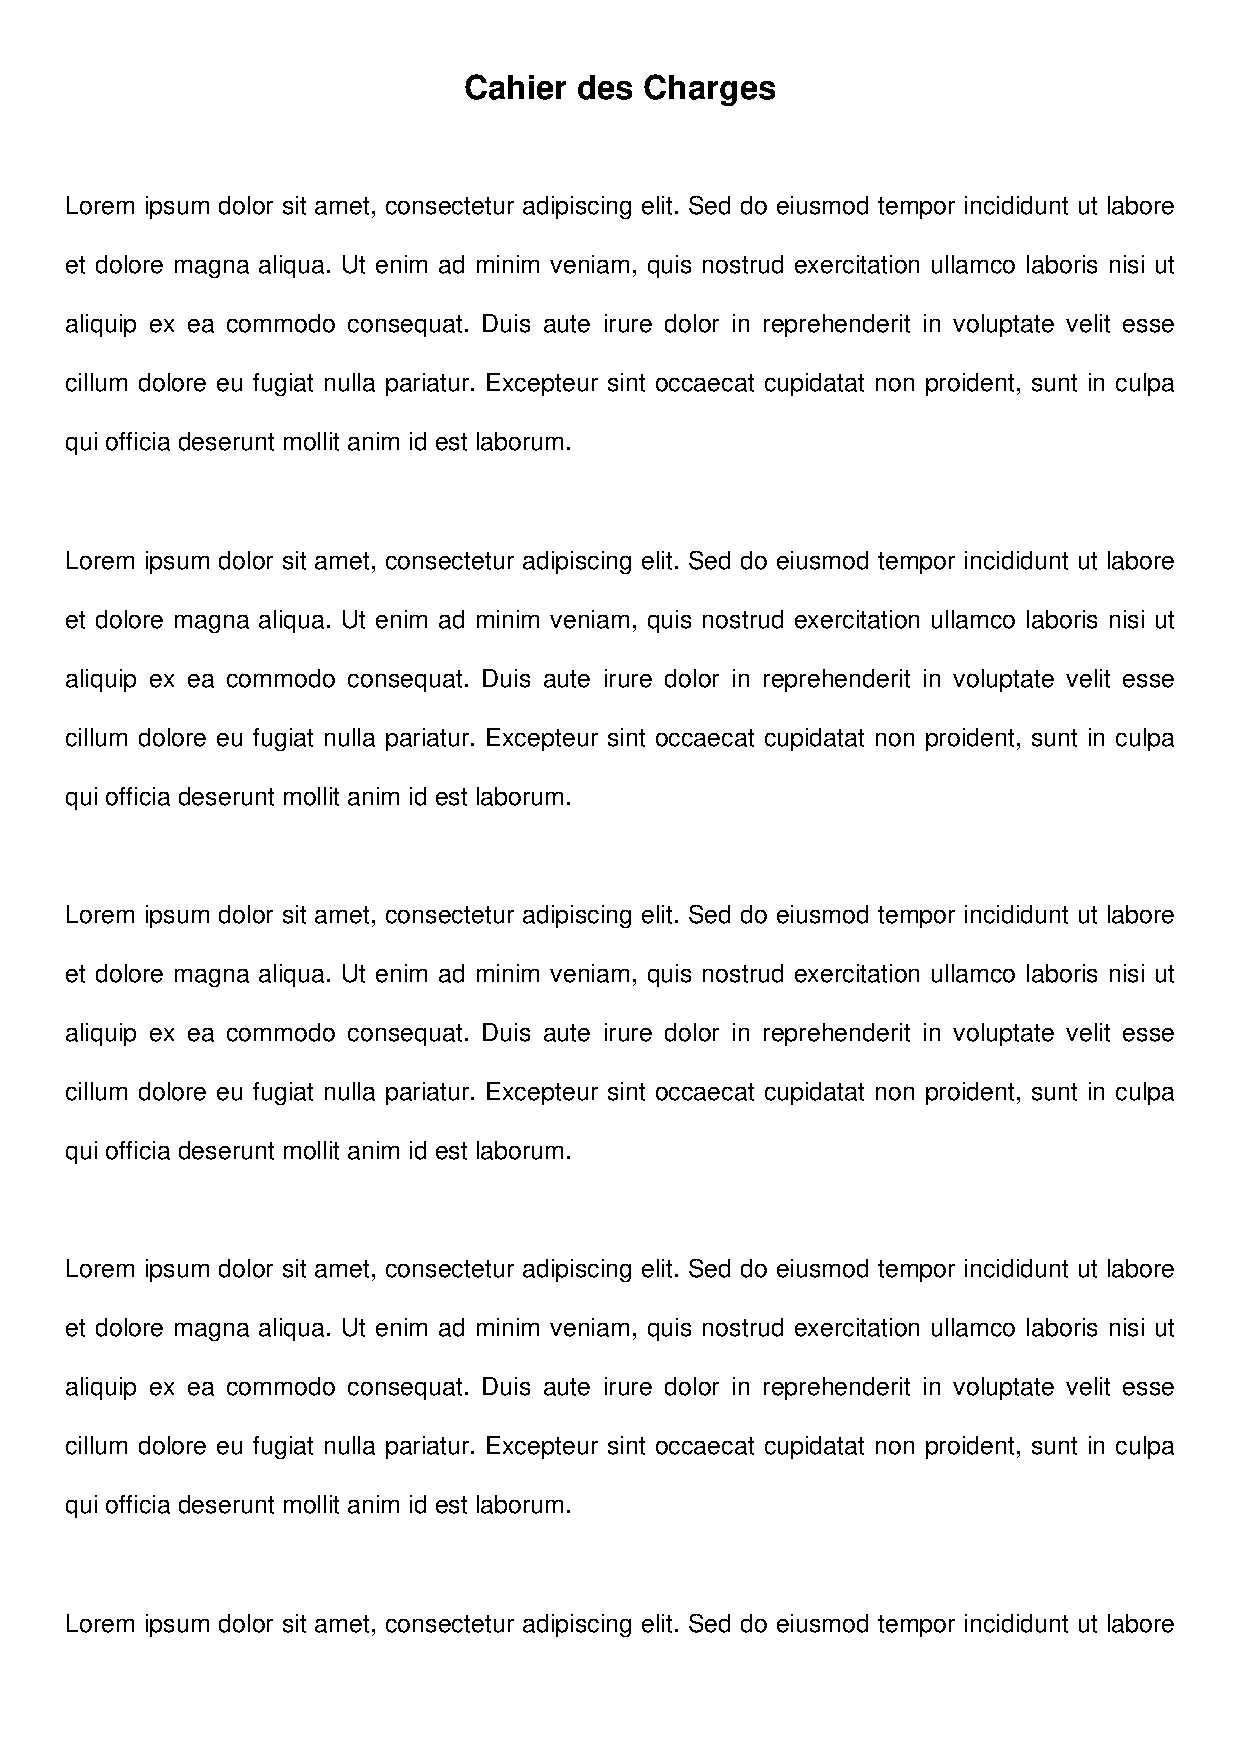
\includepdf[pages=-]{other/cahier_des_charges.pdf}







% Exemple d'utilisation de lorem ipsum
\section{Exemple d'annexe avec Lorem Ipsum}
\lipsum[1-3]

\subsection{Sous-annexe avec Lorem Ipsum}
\lipsum[4-6]


%\appendix
%
%\renewcommand{\thesection}{\arabic{section}}
%\renewcommand{\thesubsection}{\thesection.\arabic{subsection}}
%\renewcommand{\thetable}{\thesection.\arabic{table}}
%\renewcommand{\thefigure}{\thesection.\arabic{figure}}
%
%
%
%\newlistof{annexlist}{annextoc}{} 
%\newcommand{\annex}[1]{
%    \refstepcounter{section}
%    \section*{\thesection\hspace{1em}#1}
%    \addcontentsline{annextoc}{section}{\thesection\hspace{0.5em}#1} 
%}
%\newcommand{\subannex}[1]{
%    \refstepcounter{subsection}
%    \subsection*{\thesubsection\hspace{1em}#1}
%    \addcontentsline{annextoc}{subsection}{\thesubsection\hspace{0.5em}#1}
%}
%
%% Table des annexes
%\section*{Table des annexes}
%\vspace*{-2.5em}
%\addcontentsline{toc}{section}{Table des annexes}
%\listofannexlist
%\newpage
%
%% Exemple d'annexe
%\annex{Titre de l'annexe A}
%Contenu de l'annexe A.
%
%\subannex{Sous-annexe A.1}
%Contenu de la sous-annexe A.1.
%
%\subannex{Sous-annexe A.2}
%Contenu de la sous-annexe A.2.
%
%\annex{Titre de l'annexe B}
%Contenu de l'annexe B.
%
%\subannex{Sous-annexe B.1}
%Contenu de la sous-annexe B.1.
\end{document}